\section{Results}
\label{results}
There is a huge difference between simulating a system and running the physical platform. Often there will be policies running flawlessly in simulation but are unable to solve the problem even closely in reality. Further, the algorithms behave quite differently during their training. Thus, in order to present and discuss our findings we will split this section in two parts, Simulation and Physical System.

\subsection{Simulation}
\label{sim}

\begin{figure*}
\centering
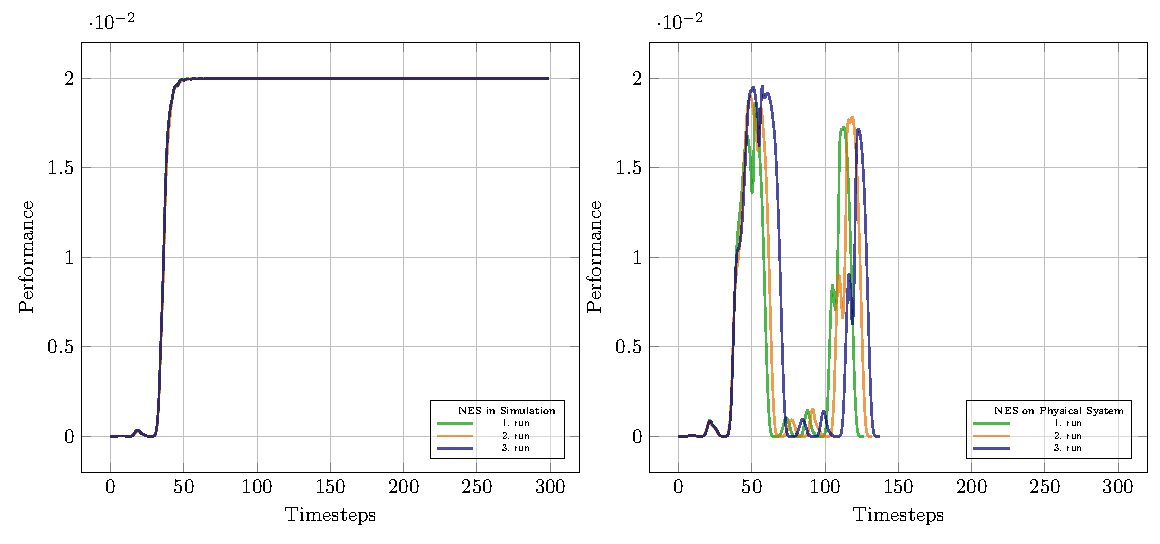
\includegraphics[scale=.6]{plots/benchmark_Qube_NES_plattforms_working.pdf}
\caption{This figure is a placeholder showing our struggles}
\label{fig:NPG_training}
\end{figure*}

Training with the NPG turned out to be quite difficult. The biggest hurdle is finding suitable hyperparameters. \autoref{fig:NPG_training} shows the training process of the NPG with two different sets of hyperparameters. For these plots we chose to change INSERT PARAMETER HERE, however this is only one of many hyperparameters that can be changed in order to solve the optimization problem. The most important of them are:
\begin{enumerate}
  \item $\delta$: \\
  Increasing $\delta$ increases the step of the policy update which can lead to faster convergence. However this can also result in worse performance because the algorithm does not converge and instead jumps between suboptimal solutions. \\
  \item $\gamma$: \\
  $\gamma$ can be used to set more focus to short or long term rewards. Increasing the value also increases the importance of long term reward and vice versa \cite{He2018}. \\
  \item $\lambda$: \\
  $\lambda$ is used to realize a tradeoff between bias and variance in the advantage estimation \cite{He2018}. \\
  \item Number of roll outs: \\
  Increasing the number of roll outs per episode decreases the variance during roll outs. \\
  \item Policy: \\
  The policy is an important factor. Depending on the tasks to solve different policies can be applied \cite{Rajeswaran2017}. For our implementation we only use a neural network representing a gaussian distribution. Thus we can only change the network size. The activation function is fixed as $tanh$, but still the size itself is already a huge factor. \\
  \item Baseline: \\
  The baseline, estimating the state-value function, is also represented with a neural network. DISCUSS size, epochs, batches, optimizer
\end{enumerate}
\begin{figure*}
\centering
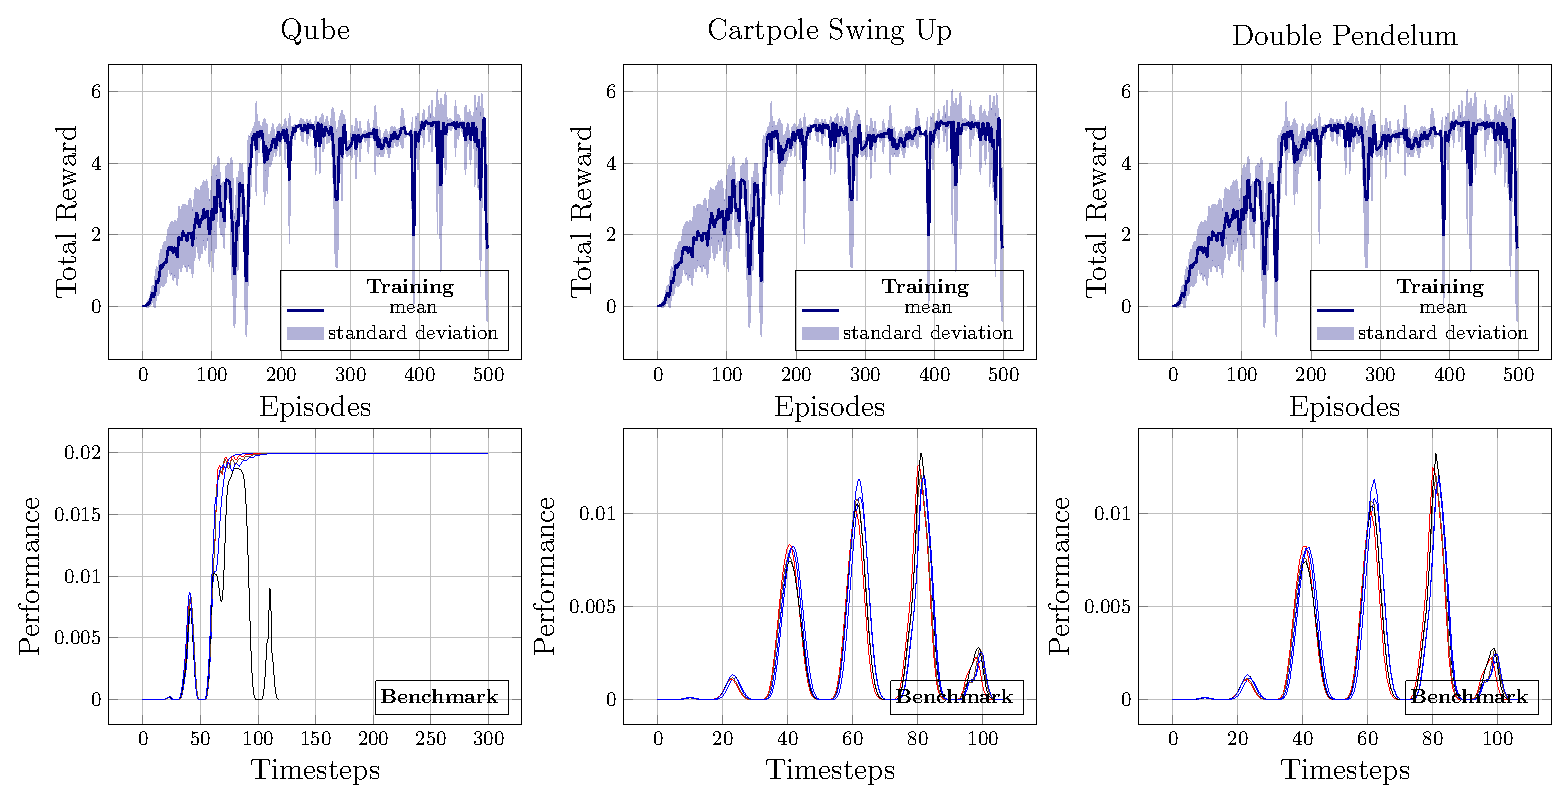
\includegraphics[scale=.4]{plots/learned_benchmarked_NPG.pdf}
\caption{This figure shows the training process of the NPG as well as a benchmark with the final policy on each of the three tasks described in \autoref{intro}. "Qube" is refering to the Furuta Pendulum.}
\label{fig:NPG_final}
\end{figure*}

\autoref{fig:NPG_final} shows our final results on the given tasks using the NPG. All of the graphs were created during simulations, which is easier in most cases because of simplifications that are usually made in the derivations of the dynamics in such systems \cite{Cazzolato2011}. As such the simulations run more smoothly and can even end up with unrealisticly good policies. We will discuss this more in \autoref{phys}. Still, we were only able to solve the Qube with the NPG. Based on the fact that we managed to solve the Qube, we assume that the algorithm was implemented correctly and we were only unable to find suitable parameters as there are a lot that can change the training process tremendously which we already described above. \\
Further as \autoref{fig:NPG_final} shows the NPG can be quite unstable during its' training process. At around 200, 600 and 700 episodes there are huge jumps in the performance. These jumps can be reduced or even be prevented by reducing the learning rate $\delta$, which in contrast also decreases convergence speed or might even cause the algorithm to get stuck in poor optima. \\
Another important insight are the benchmark plots in \autoref{fig:NPG_final}. On these plots always only three runs are shown to increase visability. In reality we did around 100 runs for each policy to verify its' performance. This was necessary because, depending on the environment, the starting position can vary. This might lead to false positive results when to few runs are performed, which can also be seen in the plots of the Cartpole tasks in \autoref{fig:NPG_final}. INSERT WHAT CAN BE SEEN ON THE PLOTS. In contrast the well trained policy performed well in all runs. During these benchmark the policies behaved greedily to ensure the best possible actions where executed. \\
During our tests, which are not shown as Figures in this report we have also seen policies converge so well that almost no exploration was left and thus the performance in the last few episodes of the training process was almost similar to the benchmark performance. This outcome is the optimal situation as in theory a gaussian policy like the one we used for this project should converge to an optimum without further exploration if it is trained long enough with suitable hyperparameters.

\begin{figure*}
\centering
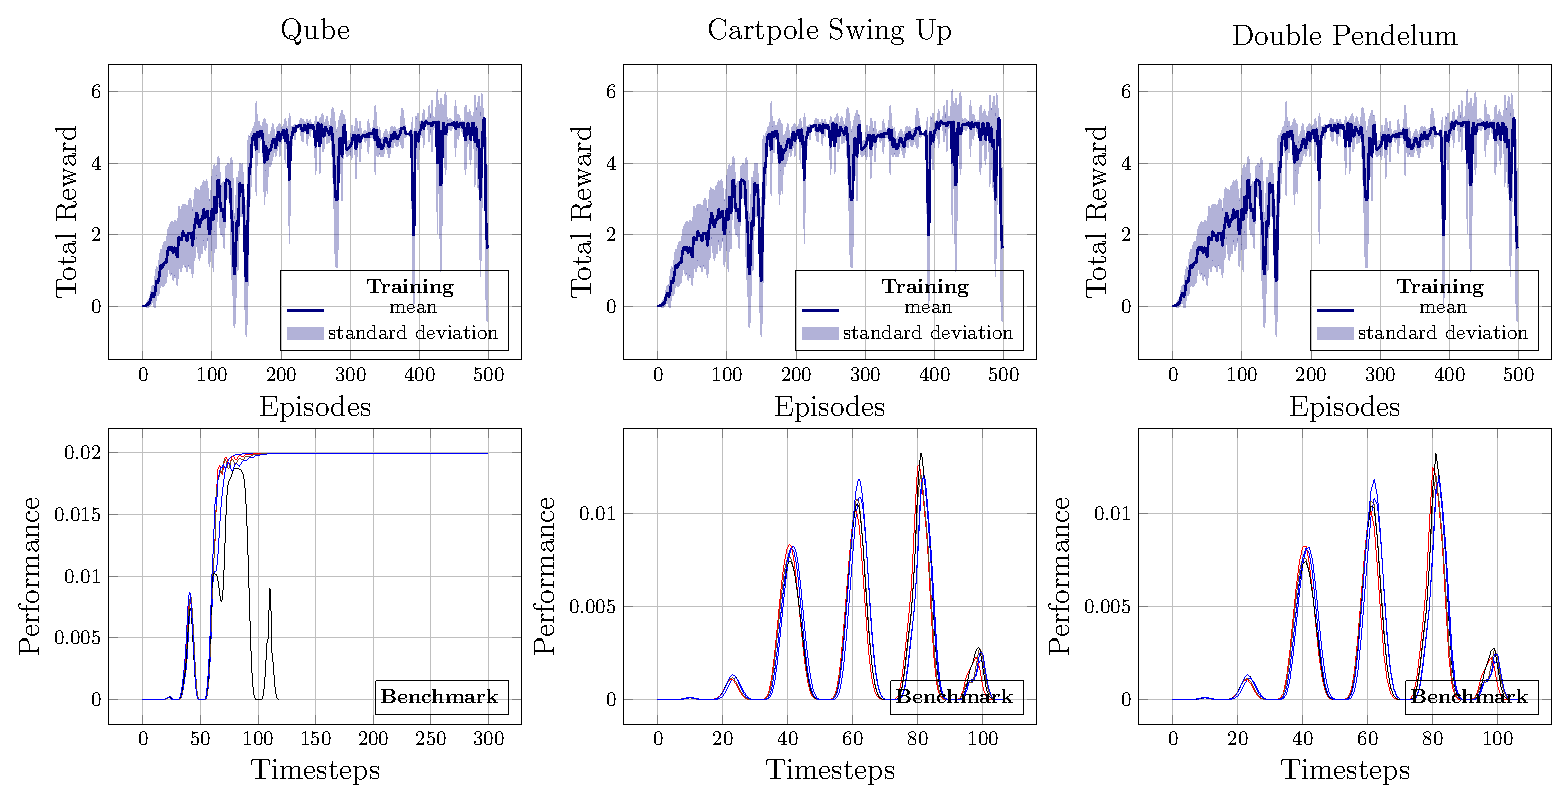
\includegraphics[scale=.4]{plots/learned_benchmarked_NPG.pdf}
\caption{This figure shows the performance of a policy trained in simulation. On the left you can see three runs done in simulation and on the right the same policy applied to the physical system}
\label{fig:NES_training}
\end{figure*}

As already described in \autoref{intro} the Canonical NES had similar problems as the first version of the NPG. Inverting the FIM often resulted in singular matrices, but in addition both were very slow. For the NPG we advanced towards TRPO in order to solve this issue. In case of the NES we decided to switch to the SNES, which turned out to be a huge success. \autoref{fig:NES_training} shows our results of the NES on all tasks. We managed to solve all platforms quite quickly with a single exception being the Furuta Pendulum. The biggest reason why is that the SNES compared to the NPG/TRPO has much less hyperparameters that need to be adjusted. The only ones being:
\begin{enumerate}
  \item $\lambda$: \\
  The population size $\lambda$ defining the amount of samples which are drawn from the search distribution for each episode. For all our solution we used the suggested calculation in \cite{Wierstra14} to set $\lambda$ which is also defined as the default setup in our project. \\
  \item Number of roll outs: \\
  In case of the NES this parameter not quite defines the number of roll outs per episode but rather the roll outs performed for each policy evaluation. Thus for each episode $n = \lambda * number \ of \ roll \ outs$ simulations are done while resetting the environment seed between each sample to a random value chosen at the beginning of each episode. Increasing the number of roll outs decreases the variance during roll outs which is identical to the NPG. For all platforms except the Furuta Pendulum this was set to one and turned out to be enough to find good solutions. To solve the Furuta Pendulum however, we had to use 15 roll outs as it was much more unstable than the cartpole. \\
  \item Policy: \\
  Similar to the NPG the policy can we varied depending of tasks and setup, but we decided to use the same policy as the NPG with the exception that only greedy evaluations are performed as the NES already incorporates exploration in the search distribution over the policy parameters. Still the neural network can be adjusted in size and activation function, which however turned out not to be as impactful as in the NPG. For all tasks we used a neural network with a single layer and 10 nodes.
\end{enumerate}

Compared to the NPG though the SNES is harder to interpret during its' training process. \autoref{fig:NES_training} shows that e.g. the Furuta Pendulum performed much worse during the last few episodes of the training process than the benchmark. We realized that the SNES takes much longer to converge to almost no exploration. Still in most tasks it managed to converge to a near optimal solution much faster than the NPG. \\

In the end the SNES was not only easier to implement but also much easier to handle and set up. It has a lot less crucial hyperparameters that need to be adjusted and in addition it is also much more invarient to small changes in the hyperparameters.

\subsection{Physical System}
\label{phys}

\begin{figure}[ht]
\centering
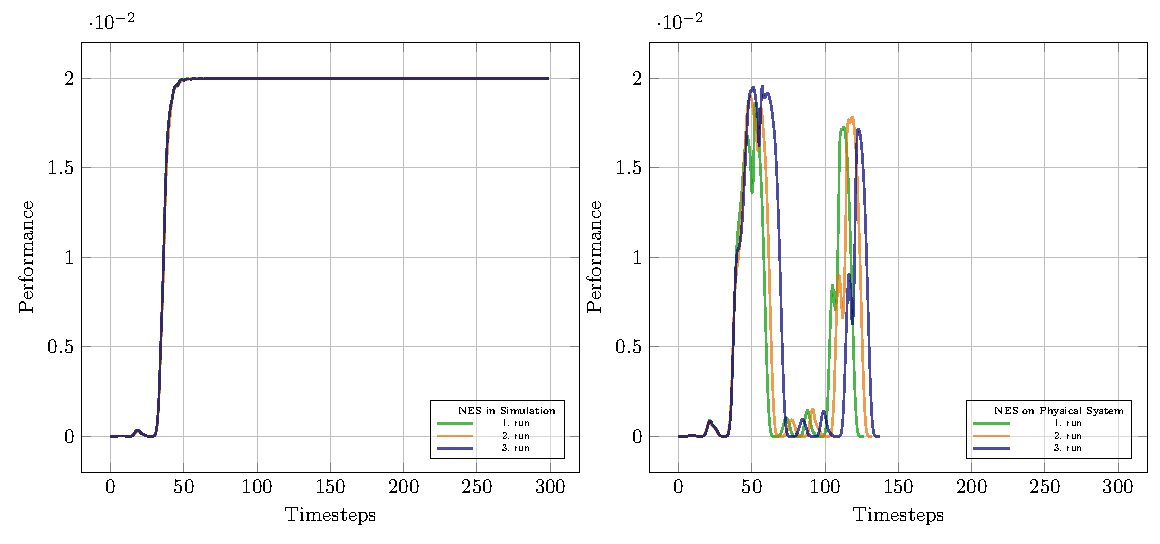
\includegraphics[scale=.6]{plots/benchmark_Qube_NES_plattforms_working.pdf}
\caption{This figure shows the performance of a policy trained in simulation. On the left you can see three runs done in simulation and on the right the same policy applied to the physical system}
\label{fig:NES_sim_to_pyhs}
\end{figure}

\begin{figure}[ht]
\centering
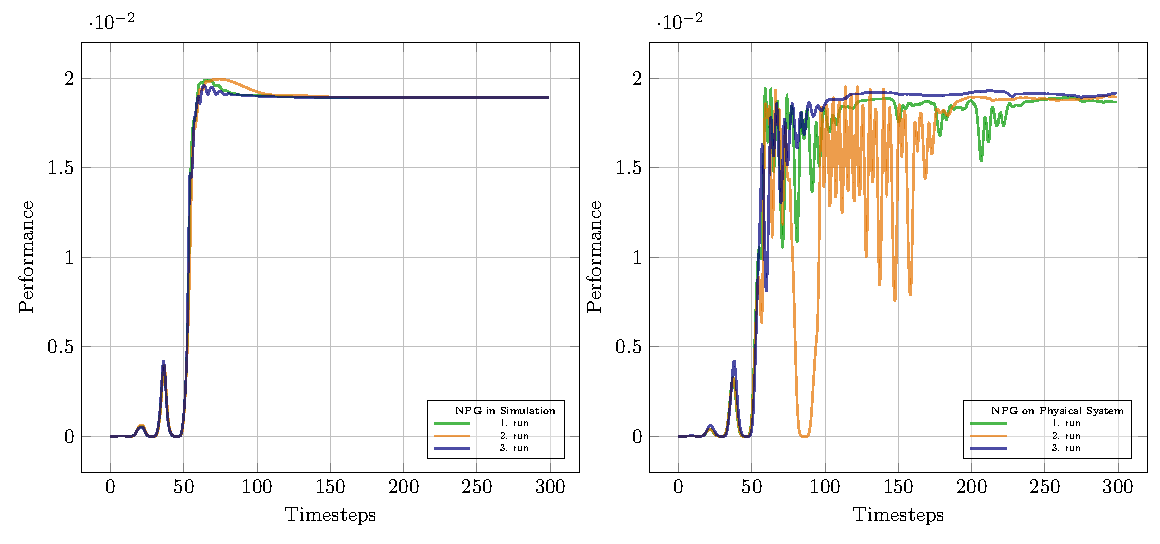
\includegraphics[scale=.6]{plots/benchmark_Qube_NPG_plattforms_working.pdf}
\caption{This figure shows the performance of a policy trained in simulation. On the left you can see three runs done in simulation and on the right the same policy applied to the physical system}
\label{fig:NPG_sim_to_pyhs}
\end{figure}
